\scanpage{25}
% Folio d'archive : 24. Feuille entièrement diagrammatique.
% Petit diagramme, angle supérieur gauche.
\diagram{\begin{tikzcd}[column sep=small,row sep=small]
 & e\arrow[d] &\Omega Z\arrow[l]\arrow[d]\\
e\arrow[d] &\Omega Y\arrow[l]\arrow[d] &\Omega X\arrow[l]\arrow[d]\\
X\arrow[d] & Z\arrow[l]\arrow[d] &e\arrow[l]\\
Y &e\arrow[l] &
\end{tikzcd}}
% Grand escalier central ; tous les e, exposants et flèches conservés.
\diagram{\begin{tikzcd}[column sep=small,row sep=small]
&&&&e\arrow[d]&\Omega^3 Z\arrow[l]\arrow[d,"\Omega^3 g"]&\Omega^4 Y\arrow[l,"\Omega^3 h"']\arrow[d]\\
&&&e\arrow[d]&\Omega^3 Y\arrow[l]\arrow[d,"\Omega^2 h"']&\Omega^3 X\arrow[l,"\Omega^3 f"']\arrow[d]&e\arrow[l]\\
&&e\arrow[d]&\Omega^2 X\arrow[l]\arrow[d,"\Omega^2 f"']&\Omega^2 Z\arrow[l,"\Omega^2 g"']\arrow[d]&e\arrow[l]&\\
&e\arrow[d]&\Omega Z\arrow[l]\arrow[d,"\Omega g"']&\Omega^2 Y\arrow[l,"\Omega h"']\arrow[d]&e\arrow[l]&&\\
e\arrow[d]&\Omega Y\arrow[l]\arrow[d,"h"']&\Omega X\arrow[l,"\Omega f"']\arrow[d]&e\arrow[l]&&&\\
X\arrow[d,"f"']&Z\arrow[l,"g"']\arrow[d]&e\arrow[l]&&&&\\
Y&e\arrow[l]&&&&&
\end{tikzcd}}
% Petit angle isolé à droite.
\diagram{\begin{tikzcd}[column sep=small,row sep=small]
&\unsure{P|P'}\arrow[d]\\
p&Q\arrow[l]
\end{tikzcd}}
% Suite commencée immédiatement au-dessous du pli horizontal.
\diagram{\begin{tikzcd}[column sep=small]
Y&X\arrow[l]&Z\arrow[l]&\Omega Y\arrow[l]&{}\arrow[l]
\end{tikzcd}}
% Esquisse en perspective, moitié inférieure gauche : flèches, cercles
% et reprises de traits sont restitués comme dessin et non interprétés.
\figure{\begin{tikzpicture}[scale=.78]
\node[draw,circle,inner sep=1pt] (a) at (2,4.4) {$e$};
\node[draw,circle,inner sep=1pt] (b) at (1,3.5) {$e$};
\node[draw,circle,inner sep=1pt] (c) at (0,2.5) {$e$};
\node[draw,circle,inner sep=2pt] (x) at (0,1.5) {$\bullet$};
\node[left] at (x.west) {$X$};
\node[draw,circle,inner sep=2pt] (y) at (0,.4) {$\bullet$};
\node[left] at (y.west) {$Y$};
\node[draw,circle,inner sep=1pt] (d) at (1,.4) {$e$};
\node[draw,ellipse,inner sep=3pt] (e) at (2.15,1.5) {$e$};
\node[draw,ellipse,inner sep=3pt] (f) at (3,2.5) {$e$};
\coordinate (g) at (1,1.5);\coordinate (h) at (1,2.5);
\coordinate (i) at (2,2.5);\coordinate (j) at (2,3.5);
\coordinate (k) at (3,3.5);
\draw[->] (a)--(b);\draw[->] (b)--(c);\draw[->] (b)--(h);
\draw[->,thick] (h)--(c);\draw[->] (c)--(x);\draw[->] (x)--(y);
\draw[->] (d)--(y);\draw[->] (g)--(d);\draw[->] (h)--(g);
\draw[->,thick] (g)--(x);\draw[->] (e)--(g);\draw[->] (e)--(d);
\draw[->] (i)--(e);\draw[->] (f)--(e);\draw[->,thick] (f)--(i);
\draw[->] (i)--(h);\draw[->] (j)--(i);\draw[->,thick] (j)--(b);
\draw[->] (k)--(j);\draw[->] (k)--(f);\draw[->] (a)--(j);
\draw[->] (j)--(g);\draw[->] (2.8,3.8)--(2.8,5.2);
\draw[->] (3.6,4.4)--(3.6,3.7);
\draw[very thick,rounded corners=3pt] (1.9,3.5)--(1.9,4.6)--(2.1,4.6)--(2.1,3.7)--(3,3.7)--(3.3,2.6)--(3.3,1.1);
\draw (1.75,3.6)--(1.8,4.8);\draw (3.1,3.6)--(3.1,.6);
\draw (.4,4.7)--(1.9,4.7);\draw (.4,4.05)--(2.8,4.05);
\draw[dashed] (2.9,4.3)--(3.5,4.3);\draw[dashed] (3.2,3.5)--(3.6,3.5);
\end{tikzpicture}}
% Deux points isolés, à droite sous la suite commencée.
\diagram{\begin{tikzcd}[column sep=small]\bullet&\bullet\end{tikzcd}}
% Deux petits carrés déformés, à droite de l'esquisse.
\diagram{\begin{tikzcd}[column sep=small,row sep=small]
e\arrow[d,thick]&{}\arrow[dd,dashed]&\bullet\arrow[ll,dashed]\\
X\arrow[d]&&e\arrow[ll,thick]\arrow[dl]\arrow[u,dotted,very thick]\\
Y&e\arrow[l]&
\end{tikzcd}}
% Longue suite inférieure avec les e intercalés ; la suite se poursuit hors dessin.
\diagram{\begin{tikzcd}[column sep=.8em,row sep=1.2em]
&&e\arrow[dl]&&e\arrow[dl]&&e\arrow[dl]&&e\arrow[dl]&&\\
Y&X\arrow[l]&Z\arrow[l]\arrow[dl]&\Omega Y\arrow[l]\arrow[ul]&\Omega X\arrow[l]\arrow[dl]&\Omega Z\arrow[l]\arrow[ul]&\Omega^2 Y\arrow[l]\arrow[dl]&\Omega^2 X\arrow[l]\arrow[ul]&\Omega^2 Z\arrow[l]\arrow[dl]&\Omega^3 Y\arrow[l]\arrow[ul]&{}\arrow[l]\\
&e\arrow[ul]&&e\arrow[ul]&&e\arrow[ul]&&e\arrow[ul]&&&
\end{tikzcd}}
% Reprise rayée sous l'extrémité gauche de la suite.
\deleted{\figure{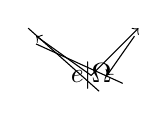
\begin{tikzpicture}
\node at (0,0) {$\unsure{e|\Omega}$};
\draw[->] (0,0)--(-.7,.5);\draw[->] (0,0)--(.6,.6);
\draw (-.7,.4)--(.4,-.1);\draw (-.8,.6)--(.1,-.2);
\draw[->] (.55,.5)--(.2,0);
\end{tikzpicture}}}
